\documentclass{article}
\usepackage[utf8]{inputenc}
\usepackage{graphicx}
\graphicspath{ {./images/} }
\usepackage{amsmath}
\usepackage{amssymb}
\usepackage[T1]{fontenc}
\usepackage{subcaption}
\usepackage{wrapfig}
\usepackage{enumitem}
\usepackage{cancel}
\usepackage{xcolor}
\newcommand\Ccancel[2][black]{\renewcommand\CancelColor{\color{#1}}\cancel{#2}}
\usepackage{bm}
\usepackage[colorlinks,bookmarks=false,linkcolor=black,urlcolor=black]{hyperref}
\usepackage{float}
\usepackage{mathtools}
\newcommand{\defeq}{\vcentcolon=}
\newcommand{\eqdef}{=\vcentcolon}
\usepackage{mathtools, stmaryrd}
\usepackage{xparse} \DeclarePairedDelimiterX{\Iintv}[1]{\llbracket}{\rrbracket}{\iintvargs{#1}}
\NewDocumentCommand{\iintvargs}{>{\SplitArgument{1}{,}}m}
{\iintvargsaux#1} %
\NewDocumentCommand{\iintvargsaux}{mm} {#1\mkern1.5mu..\mkern1.5mu#2}
\usepackage{tikz}
\usetikzlibrary{automata, positioning, arrows}
\tikzset{
->, % makes the edges directed
>=stealth, % makes the arrow heads bold
node distance=3cm, % specifies the minimum distance between two nodes. Change if necessary.
every state/.style={thick, fill=gray!10}, % sets the properties for each ’state’ node
initial text=$ $, % sets the text that appears on the start arrow
}



\title{Theory of Computation \\ Homework 2}
\author{Tom Nonnenmacher (325341),\quad Sebastian Maier (327504),\\ Sébastien Delsad (326423),\quad Jérémy Chaverot (315858).}
\date{April 2022}

\begin{document}
\maketitle

To be rigorous, one should verify that the inputs are indeed the descriptions of DFAs or TMs, using the definitions (respectively 5-tuple \& 7-tuple), because input strings can be any string in $\{0,\,1\}^\star$. This verification can always be done on finite input strings. In this homework, we assume the input is in the correct form (either DFA or TM).
\section*{Exercice 1}
Let $L_1$ denote the following language :
\begin{align*}
    L_1\; =\;\{\,\langle D,\, D'\rangle\,:\,D\;\text{and}\;D'\;\text{are DFAs and}\;L(D)\subseteq L(D')\,\}.
\end{align*}

\noindent Let us prove that the language $L_1$ is Turing-decidable, and thus is Turing-recognizable. For this purpose, we use the following equivalences : 
\begin{align*}
L(D)\subseteq L(D')\Leftrightarrow L(D)\cap L(D') = L(D)\Leftrightarrow \{L(D)\cap L(D')\}\oplus L(D)=\emptyset
\end{align*}

\noindent We give the description of a Turing machine $TM_{\text{SUBSET}}$ :
\begin{itemize}
    \item [-] get on input a pair $\langle D,\, D'\rangle$ two DFAs encoded in binary (if the input is not such a tuple, \textit{reject})
    \item [-] build a DFA $\mathcal{D}_1$ that accepts the language $L(D)\cap L(D')$ since regular languages are closed under intersection.
    \item [-] simulate $TM_{\text{EQ}}$ with $\langle D,\, \mathcal{D}_1\rangle$
    \item [-] if $TM_{\text{EQ}}$ accepts, then \textit{accept}, otherwise if $TM_{\text{EQ}}$ rejects, then \textit{reject}.
\end{itemize}

\noindent \\ The Turing machine $TM_{\text{EQ}}$, that verifies whether two DFAs accept exactly the same language or not, is constructed as follows : 
\begin{itemize}
    \item [-] get on input a pair $\langle D,\, D'\rangle$ two DFAs encoded in binary (if the input is not such a tuple, \textit{reject})
    \item [-] build a DFA $\mathcal{D}_2$ that accepts the language $L(D)\oplus L(D')$, that is equivalent to $\{L(D)\cap \overline{L(D')}\}\cup\{\overline{L(D)}\cap L(D')\}$, since regular languages are closed under complement, intersection and union.
    \item [-] simulate $TM_{\text{EMPTY}}$ with $\langle\mathcal{D}_2\rangle$
    \item [-] if $TM_{\text{EMPTY}}$ accepts, then \textit{accept}, otherwise if $TM_{\text{EMPTY}}$ rejects, then \textit{reject}.
\end{itemize}

\noindent \\ The Turing machine $TM_{\text{EMPTY}}$, that verifies whether the language of a DFA is empty or not, is constructed as follows : 
\begin{itemize}
    \item [-] get on input a singleton $\langle D\rangle$ a DFA encoded in binary (if the input is not such a tuple, \textit{reject})
    \item [-] given $\langle D\rangle$ with $D = (Q,\, \Sigma,\, \delta,\, q_0,\, F)$ 
    \begin{enumerate}
        \item Initialize $R = \{q_0\}$
        \item For each $q\in R$ and $q'\in Q\setminus R$, check if there exists a transition of the form $\delta$($q$, $a$) = $q'$ for some $a\in\Sigma$.
        \item If at least one such $q'$ is found, add $q'$ to $R$ and go back to step 2.
        \item \textit{Accept} iff $R\cap F=\emptyset$.
    \end{enumerate}
\end{itemize}

\noindent \\ All of this is summarized in the figures below.

\begin{figure}[ht] % ’ht’ tells LaTeX to place the figure ’here’ or at the top of the page
\centering
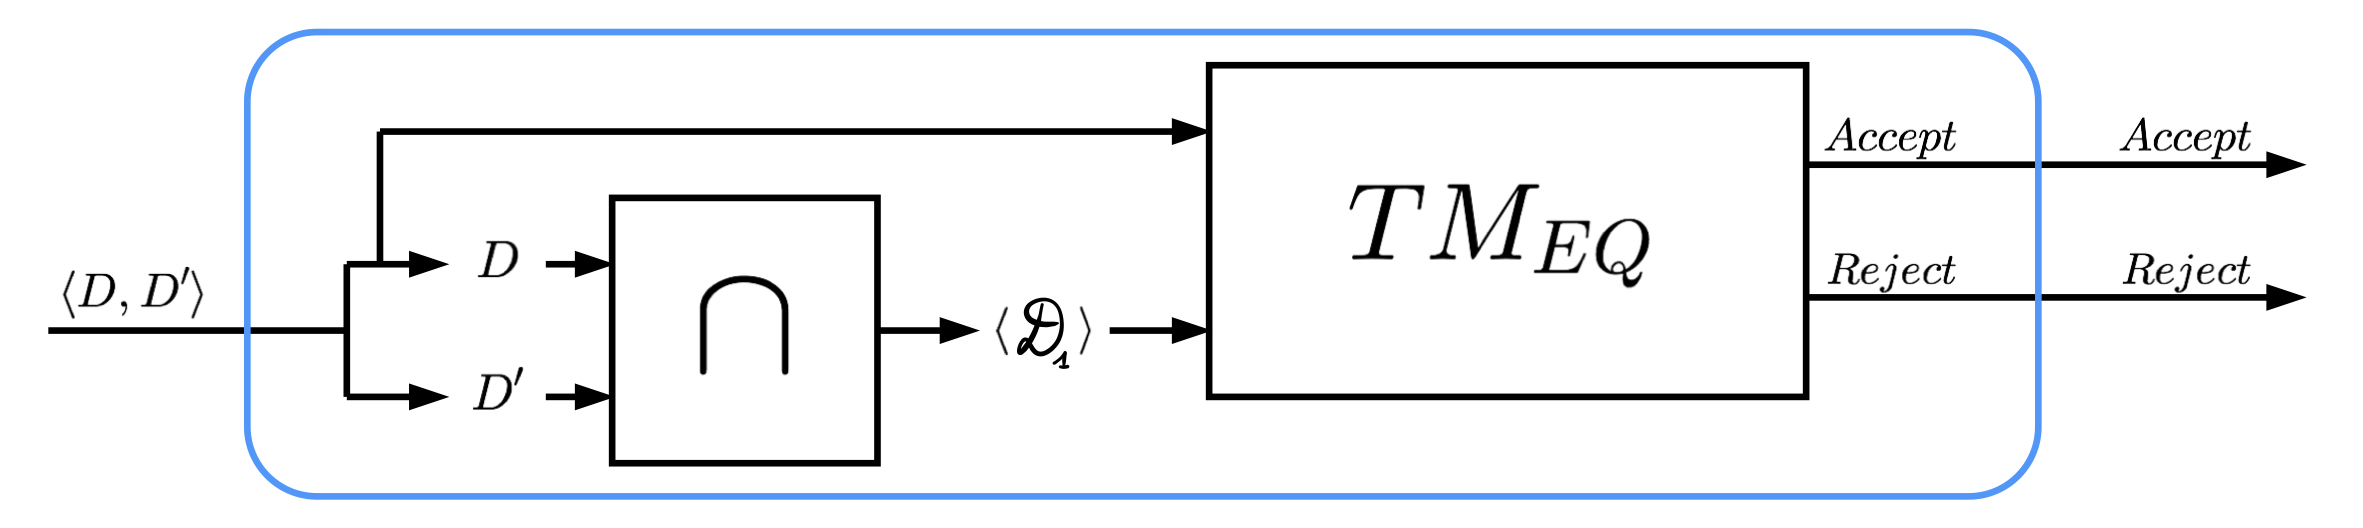
\includegraphics[scale=0.145]{images/tm subset.jpeg}
\caption{Caption of Turing machine $TM_{\text{SUBSET}}$}
\label{fig:my_label1}
\end{figure}

\begin{figure}[ht] % ’ht’ tells LaTeX to place the figure ’here’ or at the top of the page
\centering
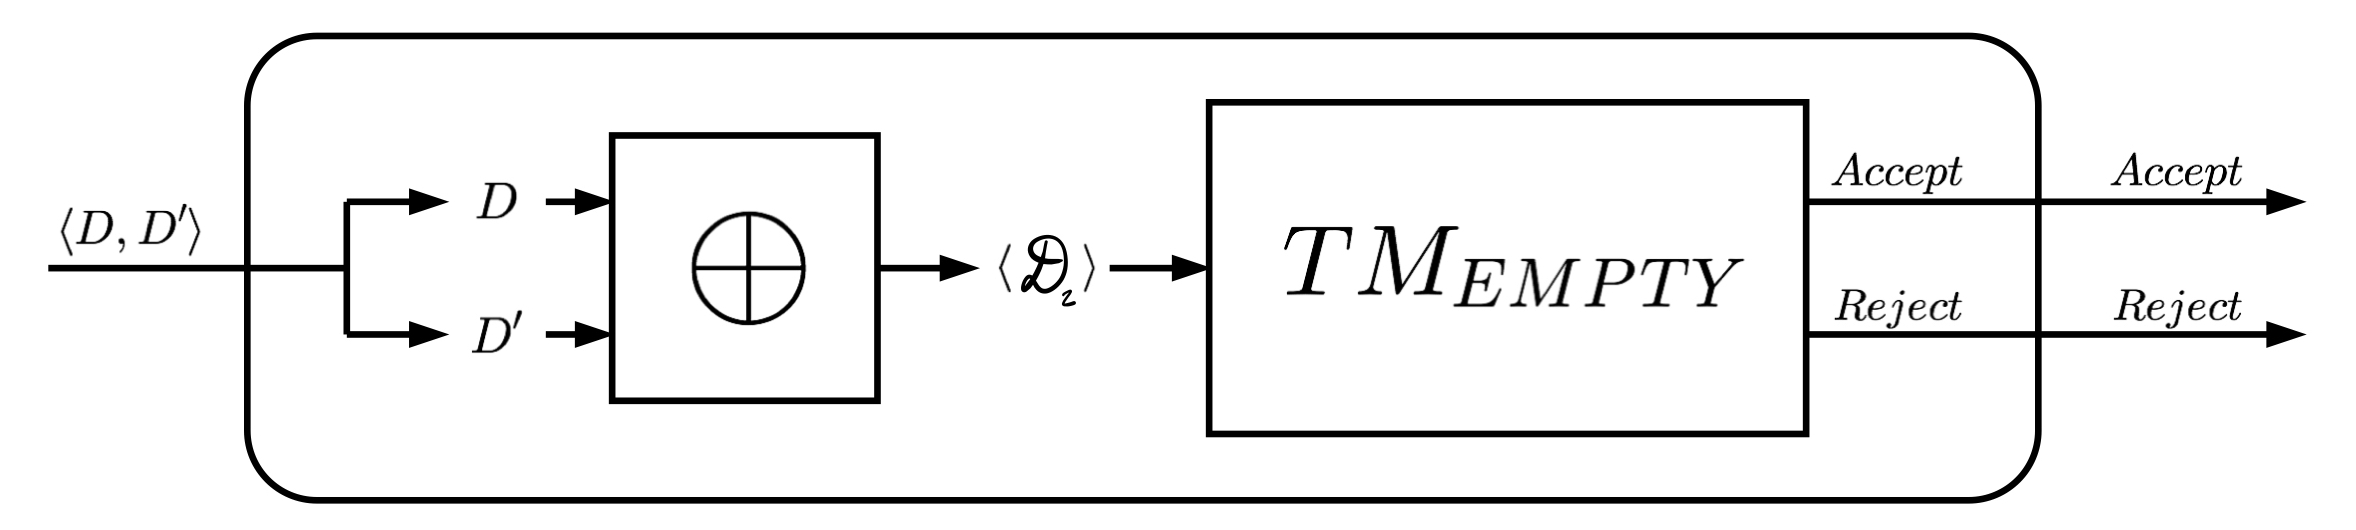
\includegraphics[scale=0.145]{images/tm eq.jpeg}
\caption{Caption of Turing machine $TM_{\text{EQ}}$}
\label{fig:my_label2}
\end{figure}

\noindent \\This completes our construction, and $TM_{\text{SUBSET}}$ decides $L_1$ (and also recognizes $L_1$ as a consequence).



\newpage
Let $L_2$ denote the following language :
\begin{align*}
    L_2\; =\;\{\,\langle M\rangle\,:\,M\;\text{is a TM and}\;L(M)\;\text{is infinite}\,\}.
\end{align*}

Let us show the unrecognizability of $L_2$.
First of all, we give the definition of the language $A_{TM}$ :
\begin{align*}
    A_{TM}\;=\;\{\,\langle M,\,w\rangle\,:\,M\;\text{is a TM and}\;M\;\text{accepts}\;w\,\} 
\end{align*}
It was shown in class that this language is Turing-undecidable (proof by contradiction using diagonalization), but it is easy to convince ourselves it is Turing-recognizable, using the following TM :

\begin{itemize}
\item [] On input $\langle M,\,w\rangle$ where $M$ is a TM and $w$ is a string :
    \begin{enumerate}
        \item Simulate $M$ on input $w$.
        \item If $M$ ever accepts, \textit{accept}. 
        \item If $M$ does not accept $w$, then \textit{reject} or \textit{loop}.
        \item This is why this TM is only a recognizer, not a decider.
    \end{enumerate}
\end{itemize}
This implies that $\overline{A_{TM}}$ is not Turing-recognizable.
Now, it is enough to show that language $\overline{A_{TM}}$ mapping reduces to language $L_2$, written $\overline{A_{TM}}\le_m L_2$. Below we present a suitable reduction.

\begin{itemize}
    \item We define a function $f(\langle T,\,w\rangle)=\langle M\rangle$, where $M$ is a TM which performs the following :
    \begin{enumerate}
        \item On input $x$, simulate $T$ with $w$ \textcolor{red}{for |x| steps}.
        \item If $T$ accepts $w$, go into an \textit{infinite loop}.
        \item Otherwise \textit{accept} $x$.
    \end{enumerate}
\end{itemize}

\noindent Thus, we have that :
\begin{itemize}
    \item If $T$ accepts $w$ (namely $\langle T,\,w\rangle\notin\overline{A_{TM}}$), the language of $M$ is empty (it accepts no string) and in particular $\langle M\rangle\notin L_2$.
    \item If $T$ does not accept $w$ (namely $\langle T,\,w\rangle\in\overline{A_{TM}}$), the language of $M$ is infinite (it accepts all strings) and in particular $\langle M\rangle\in L_2$.
\end{itemize}
Consequently we obtain the equivalence $\langle T,\,w\rangle\in\overline{A_{TM}}\;\Leftrightarrow\; f(\langle T,\,w\rangle)\in L_2$, and $f$ is a \textit{computable} function.

Therefore, it is a valid reduction, i.e. $\overline{A_{TM}}\le_m L_2$, and we can infer $L_2$ is Turing-unrecognizable (and is also Turing-undecidable as a consequence).

\newpage
\section*{Exercice 2}
Let $A$ and $B$ be two disjoint languages (i.e. $A\cap B =\emptyset$). Say that a language $C$ \textit{separates} $A$ and $B$ iff $A\subseteq C$ and $B\subseteq \overline{C}$. 
\paragraph{$\mathbf{2a}$} Suppose that $A$ and $B$ are co-Turing-recognizable (that is, $\overline{A}$ and  $\overline{B}$ are Turing-recognizable). 
Let us show that there is a Turing-decidable language $C$ that separates $A$ and $B$.\newline\linebreak 
To this end, we define two TMs $\mathcal{M}_1$ and $\mathcal{M}_2$ recognizing $\overline{A}$ and $\overline{B}$ respectively. Let $\mathcal{T}$ be a Turing machine which performs the following on input $x\,\colon$

\begin{enumerate}[noitemsep, topsep=0pt]
    \item Simulate $\mathcal{M}_1$ and $\mathcal{M}_2$ on $x$ in \textit{parallel}, that means by alternating the steps of the two TMs.
    \item If $\mathcal{M}_1$ accepts first, \textit{reject}. If $\mathcal{M}_2$ accepts first, \textit{accept}.
\end{enumerate}
By assumption, we have that $A\cap B =\emptyset$, which is equivalent to $\overline{A}\cup \overline{B} =\Sigma^\star$, and this forces the TM $\mathcal{T}$ to halt for all input $x$. So at the end, either $\mathcal{M}_1$ or $\mathcal{M}_2$ will accept the input $x$. We denote C the language decided by the TM $\mathcal{T}$, and we have that :
\begin{itemize}[noitemsep, topsep=0pt]
    \item If $x\in A$, $x$ will not be recognized by $\mathcal{M}_1$ and will be accepted by $\mathcal{M}_2$ first. Hence $A\subseteq C$.
    \item If \Ccancel[red]{$x\notin A\Rightarrow$} $x\in B$, $x$ will not be recognized by $\mathcal{M}_2$ and will be accepted by $\mathcal{M}_1$ first. Hence $B\subseteq\overline{C}$.
\end{itemize}

\noindent Therefore, this completes our construction of a decidable language $C$ that
\linebreak separates $A$ and $B$.

\paragraph{$\mathbf{2b}$} Define two disjoint languages by :
\begin{itemize}
    \item [] $A=\{\,\langle M,\,w\rangle\,:\,M\,\text{is a TM and}\,M\,\text{accepts}\,w\,\}$,
    \item [] $B=\{\,\langle M,\,w\rangle\,:\,M\,\text{is a TM and}\,M\,\text{rejects}\,w\,\}$.
\end{itemize}
We prove that there does not exist any Turing-decidable language $C$ that separates $A$ and $B$, that is for all language $C$ separating $A$ and $B$, $C$ is always non-Turing-decidable.

It appears that $A$ and $B$ are Turing-undecidable but Turing-recognizable, since for both of them it is possible to build a TM recognizing them (c.f. the language $A_{TM}$ in exercice 1). 




Note that given the definitions of $A$ and $B$, the two languages are not \textit{exhaustive} because there exist TMs that neither accept nor reject $w$\linebreak (a looping behavior for exemple), hence $A\cup B \neq\Sigma^\star$.

We consider $U=\overline{A\cup B}= \overline{A}\cap\overline{B}$. As a Turing machine can only accept, reject or loop, the language $U$ is such that :
\begin{align*}
U=\{\,\langle M,\,w\rangle\,:\,M\,\text{is a TM and}\,M\,\text{loops on}\,w\,\}   
\end{align*}
Indeed, it does not contain the TMs that accept $w$ (actually $A$), and it does not contain the TMs that reject $w$ (actually B) so it can only contain language that loop on $w$.

Now, consider $C$ that separates $A$ and $B$, i.e. $A\subseteq C$ and $B\subseteq\overline{C}\Rightarrow C\subseteq\overline{B}$. Thus we have that $C=A\cup V$ where $V$ is a language such that $V\subseteq U$.
\paragraph{First case} Let $V=\emptyset$. Hence $C=A\cup\emptyset =A$. As we know, A is in fact exactly $A_{TM}$ which is Turing-undecidable. So $C$ is Turing-undecidable.
\paragraph{Second case} Let $V\neq\emptyset$. Then $C$ is a language such that :
\begin{align*}
C=\{\,\langle &M,\,w\rangle\,:\,M\,\text{is a TM and}\,M\,\text{accepts}\,w\,\}\\
&\cup\,\{\,\langle M,\,w\rangle\,:\,M\,\text{is a TM and}\,M\,\text{loops on}\,w\,\} 
\end{align*}
Which is similar to :
\begin{align*}
    C=\{\,\langle M,\,w\rangle\,:\,M\,\text{is a TM and}\,M\,\text{accepts}\,w\,\text{or}\,M\,\text{loops on}\,w\,\}
\end{align*}
As $V\neq\emptyset$, there exist TMs in $C$ which loop on a string, and as we cannot decide if a TM can loop on a string, that means $C$ is undecidable. Quod Erat Demonstrandum.\linebreak

Here is the scheme of another proof.
Suppose towards contradiction that there exists a decidable language $C$ that separates $A$ and $B$. We denote $\mathcal{D}$ the TM which is a decider for $C$, and performs as follows on input string $x$:
\begin{itemize}[noitemsep, topsep=0pt]
    \item [1.] Get its own binary description $\langle\mathcal{D}\rangle$.
    \item [2.] Simulate $\mathcal{D}$ on $w$.
    \item [3.] Verify if $\langle\mathcal{D},\,w\rangle$ belongs to $C$. If it's the case, \textit{reject}. If not, \textit{accept}.
\end{itemize}
If the decider $\mathcal{D}$ accepts the input $w$, it means $\langle\mathcal{D},\,w\rangle\in A \subseteq C$, however $\mathcal{D}$ rejects $w$ then. If the decider $\mathcal{D}$ rejects the input $w$, it means $\langle\mathcal{D},\,w\rangle\in B \subseteq \overline{C}$, however $\mathcal{D}$ accepts $w$ then. It is obviously a contradiction and the language $C$ cannot be decidable.

\noindent\newline [...]
\fi
\end{document}
